

\documentclass[a4paper,twoside,openright,titlepage,
               headinclude,,footinclude,BCOR5mm,
               numbers=noenddot,cleardoublepage=empty,
               tablecaptionabove]{scrreprt}
\usepackage[T1]{fontenc}
\usepackage[utf8]{inputenc}
\usepackage[english]{babel}
\usepackage{amsmath,amssymb}
\usepackage{indentfirst}
\usepackage[style=philosophy-modern,hyperref]{biblatex}
\usepackage{chngpage}
\usepackage{graphicx}
\usepackage{calc}
\usepackage{listings}
\usepackage{graphicx}
\usepackage{subfig}
\usepackage{lipsum}
\usepackage{shapepar}
\usepackage{pifont}
\usepackage[eulerchapternumbers,subfig,beramono,eulermath,pdfspacing,listings]{classicthesis}
\usepackage{arsclassica}
\usepackage{microtype}
\usepackage{classicthesis}
\usepackage{comment}
\usepackage{makeidx}
\usepackage[tight,english]{minitoc}
\usepackage{mathtools,amsthm,amsfonts,amssymb}
\usepackage{bm}
\usepackage{braket}
\usepackage[font=footnotesize, labelfont={sf,bf}]{caption}
\usepackage{booktabs}
\usepackage{enumitem}
    \renewcommand{\labelenumi}{(\roman{enumi})}
\usepackage{xspace}
\usepackage{comment}

% ********************************************************************
% Personal commands
% ******************************************************************** 
\newcommand{\myTitle}{R for data science}
\newcommand{\mySubtitle}{}
\newcommand{\myName}{Gennaro Tedesco}

%% some more newcommands
\newcommand{\ie}{i.\,e.}
\newcommand{\Ie}{I.\,e.}
\newcommand{\eg}{e.\,g.}
\newcommand{\Eg}{E.\,g.} 


\DeclareRobustCommand*{\clsname}[1]{{\normalfont\sffamily#1}}
\DeclareRobustCommand*{\pkgname}[1]{{\normalfont\sffamily#1}}
\DeclareRobustCommand*{\optname}[1]{{\normalfont\ttfamily#1}}
\DeclareRobustCommand*{\cmdname}[1]{\mbox{\lstinline[basicstyle=\normalsize\ttfamily]!\\#1!}}
\DeclareRobustCommand*{\classicthesis}{Classic\-Thesis}
\DeclareRobustCommand*{\arsclassica}{{\normalfont\sffamily ArsClassica}}


% ********************************************************************
% Hyper-references
% ******************************************************************** 
\newcommand{\mail}[1]{\href{mailto:#1}{\texttt{#1}}}

% ********************************************************************
% Graphics
% ********************************************************************
\graphicspath{{Graphics/}}


% ********************************************************************
% Code
% ********************************************************************
\definecolor{lightergray}{gray}{0.99}

\lstset{language=[LaTeX]Tex,
     keywordstyle=\color{RoyalBlue},
     basicstyle=\small\ttfamily,
     commentstyle=\color{Emerald}\ttfamily,
     stringstyle=\rmfamily,
     numberstyle=\scriptsize,
     showstringspaces=false,
     breaklines=true,
     frame=lines,
     backgroundcolor=\color{lightergray},
     flexiblecolumns=true,
     escapeinside={�*}{*�},
     firstnumber=last,
} 

\newcommand{\meta}[1]{$\langle${\normalfont\itshape#1}$\rangle$}

\lstset{	morekeywords=%
    {ProvidesPackage,RequirePackage,areaset,ifthenelse,%
     chapterNumber,undefined,boolean,DeclareRobustCommand,%
     spacedallcaps,textssc,MakeTextUppercase,lehead,%
     microtypesetup,textls,spacedlowsmallcaps,MakeTextLowercase,%
     sodef,allcapsspacing,lowsmallcapsspacing,thesection,%
     color,headmark,rohead,headfont,pnumfont,titleformat,%
     part,partname,thepart,chapter,thechapter,titlerule,%
     subsection,thesubsection,subsubsection,thesubsubsection,%
     paragraph,theparagraph,descriptionlabel,titlespacing,%
     formatchapter,textcolor,clearscrplain,rofoot,labelitemi,
     captionsetup,hypersetup}}

\lstnewenvironment{code}% 
   {\setkeys{lst}{columns=fullflexible,keepspaces=true}%
   \lstset{basicstyle=\small\ttfamily}}{}


% ********************************************************************
% Bibliography
% ******************************************************************** 
\bibliography{Bibliography}

\defbibheading{bibliography}{%
\cleardoublepage
\manualmark
\phantomsection
\addcontentsline{toc}{chapter}{\tocEntry{\bibname}}
\chapter*{\bibname\markboth{\spacedlowsmallcaps{\bibname}}
{\spacedlowsmallcaps{\bibname}}}}

\renewcommand*{\nameyeardelim}{\addcomma\space}

\makeindex

% -------- new commands defined below -----------
\newcommand{\df}{\texttt{data.frame}\xspace}

% equations labelled within the sections
\numberwithin{equation}{section}

%newtheoremstyle
\newtheoremstyle{classicthm}
{15pt}
{15pt}
{\rmfamily}
{}
{\itshape}
{:}
{.5em}
{}


\begin{document}
\pagestyle{plain}
% !TEX TS-program = pdflatex
% !TEX root = ../ArsClassica.tex

%*******************************************************
% Titlepage
%*******************************************************
\begin{titlepage}
\pdfbookmark{Titlepage}{Titlepage}
\changetext{}{}{}{((\paperwidth  - \textwidth) / 2) - \oddsidemargin - \hoffset - 1in}{}
    \begin{center}
        \large  

        \hfill

        \vfill

        \begingroup
            \color{Maroon}\spacedallcaps{\myTitle} \\ \bigskip
        \endgroup

        %\spacedallcaps{\myName}

        \vspace{2cm}

        
\includegraphics[scale=3]{Graphics/logo} \\ 
        
        \vspace{3cm}
        Dissertation\\ 
        zur Erlangung des mathematisch-naturwissenschaftlichen
        Doktorgrades \\``Doctor rerum naturalium''der Georg-August-Universit\"at 
        G\"ottingen  
        
        \bigskip
        im Promotionsprogramm ProPhys\\ 
        der Georg-August University School of Science (GAUSS) 
        
        \vspace{1cm}       
        vorgelegt von\\
        \myName \\
        aus Eboli, Italy\\
        
        \vspace{1cm}
        
        G\"ottingen, 2014
        %\mySubtitle \\ \medskip   
        %\myDegree \\
        %\myDepartment \\ \medskip       
        
        %\myFaculty \\ \medskip
        
        %\myUni \\ \bigskip

        %\myTime\ %-- \myVersion

        \vfill               

    \end{center}        
\end{titlepage} 
\pagestyle{scrheadings}
\dominitoc

%********************************************************************
% Mainmatter
%*******************************************************
%************************************************
\chapter{Introduction}\label{sec: pre}
%************************************************
\noindent In the following a quick guide to
common features of some \texttt{R} packages
is shown. It is by no means intended to be a guide
to the language, rather an introductory
primer to some libraries useful in data 
science for the ones who are already 
familiar with the language. 

As best practice, the reader is always
addressed to the official documentation; 
moreover, given any \texttt{R} function, the 
line \texttt{?<function>} prompts the corresponding
definitions and in-built help.
\bigskip

A full list of functions according to the package 
they are defined in is available here.\footnote{ 
\url{http://www.rdocumentation.org/}}

\bigskip 

Unless specified otherwise, minimal working examples
are shown by making use of the sample datasets provided
by \texttt{R}, in particular we will mainly refer to
\texttt{data(iris)}, \texttt{data(mtcars)} and \texttt{data(morley)}. 
We will henceforth refer to a generic data frame as to \texttt{df}.
Another set of data we will make use of is the following
quark\label{quark} data set: 
\begin{verbatim}
set.seed(1)
lab      <- sample (LETTERS[1:6], 100, replace = TRUE) 
flavour  <- sample(c("up", "down", "charme", "strange", 
		"top", "bottom"), 100, replace = TRUE)
S_z      <- sample(c("1/2", "-1/2"), 100, replace = TRUE)
quarks   <- data.table(lab, flavour, S_z)

R: head(quarks, 5)

   lab flavour  S_z
1:   B strange  1/2
2:   C  charme  1/2
3:   D    down -1/2
4:   F  bottom  1/2
5:   B strange  1/2
\end{verbatim}


%************************************************
\chapter{Vectorised operations on data frames}\label{sec: apply}
%************************************************
Given a data frame, the functions of the family
\texttt{apply} allow to perform vectorised operations
on rows and columns thereof, without having the manually
access each entry to loop through.

\section{apply}
The general wrapper for such operations is the
\texttt{apply} function, where rows and columns can 
be accessed specifying the labels $(1,2,\ldots)$ (and higher 
if any other multi-dimensional object is contained 
therein). It returns a vector (or a list) of 
values obtained by applying a function to the 
rows (columns, respectively) of a data frame, coerced
to matrix first. The general syntax is 
\texttt{apply(df, margin, FUN = <function> )}, with \texttt{margin} being
$1,2,\ldots$ and \texttt{<function>} being any function.
\begin{verbatim}
R: cars <- head(mtcars[,1:7],4)
R: cars
                   mpg cyl disp  hp drat    wt  qsec
Mazda RX4         21.0   6  160 110 3.90 2.620 16.46
Mazda RX4 Wag     21.0   6  160 110 3.90 2.875 17.02
Datsun 710        22.8   4  108  93 3.85 2.320 18.61
Hornet 4 Drive    21.4   6  258 110 3.08 3.215 19.44

# choose 1 for rows
R: apply(cars, 1, mean)

Mazda RX4  Mazda RX4 Wag     Datsun 710 Hornet 4 Drive 
45.71143       45.82786       36.08286       60.16214 
      
# choose 2 for columns
R: apply(cars, 2, mean)  

    mpg      cyl     disp       hp     drat       wt     qsec 
21.5500   5.5000 171.5000 105.7500   3.6825   2.7575  17.8825
\end{verbatim}
In the simple cases of the function being the sum or the mean,
specific operators exist as \texttt{colSums} and \texttt{colMeans},
and equivalently for rows:
\begin{verbatim}
R: colSums(cars)

   mpg    cyl   disp     hp   drat     wt   qsec 
 86.20  22.00 686.00 423.00  14.73  11.03  71.53
 
R: rowMeans(cars)

Mazda RX4  Mazda RX4 Wag     Datsun 710 Hornet 4 Drive 
45.71143       45.82786       36.08286       60.16214 
\end{verbatim}

\section{lapply and sapply}
\texttt{lapply} applies a function to each element of a list
and returns a list back. Equivalently, \texttt{sapply} does
the same job but returns a vector back instead. As a data 
frame can be seen as a list of columns, one can have
\begin{verbatim}
R: head(quarks)

   lab flavour  S_z
1:   B strange  1/2
2:   C  charme  1/2
3:   D    down -1/2
4:   F  bottom  1/2
5:   B strange  1/2
6:   F    down -1/2

R: lapply(quarks, mode)
$lab
[1] "C"

$flavour
[1] "strange"

$S_z
[1] "1/2"

R: sapply(quarks, mode)

lab   flavour       S_z 
"C" "strange"     "1/2"
\end{verbatim}

\section{Vectorised assignments}
Vectorised assignments in \texttt{R} commute with 
functions, namely the operator \texttt{c} is such
that \texttt{c(f) = f(c)}.
\begin{verbatim}
f <- function(x) sin(x) - cos(2*x)

set.seed(1234)
x <- f(c(rnorm(5)))

set.seed(1234)
y <- c(f(rnorm(5)))

x == y

[1] TRUE TRUE TRUE TRUE TRUE
\end{verbatim}
Likewise, \texttt{ifelse} evaluates a given 
condition on each element of a vector, thus 
replacing an entire loop: the two examples 
below are indeed equivalent, the latter sparing
memory and being faster
\begin{verbatim}
set.seed(1234)
x <- rnorm(5)

R: for(i in seq(1:length(x))){
      if(x[i] < 0){
        print("negative")
      } else {
        print("positive")
      }
    }

[1] "negative"
[1] "positive"
[1] "positive"
[1] "negative"
[1] "positive"


R: ifelse(x < 0, "negative", "positive")

[1] "negative" "positive" "positive" "negative" "positive"
\end{verbatim}
The function \texttt{cumsum} returns the cumulative 
sums of values elementwise, easily replacing a 
loop through:
\begin{verbatim}
set.seed(1234)
x <- rnorm(5)

R: x
[1] -1.2070657  0.2774292  1.0844412 -2.3456977  0.4291247

R: cumsum(x)
[1] -1.2070657 -0.9296365  0.1548047 -2.1908930 -1.7617683
\end{verbatim}
\enlargethispage{\baselineskip}
As a more general result, given a vector of 
values, the operator \texttt{Reduce}
applies a function on pairs of values at 
a time, defined as
\begin{verbatim}
Reduce(f, x) = ...f(f(f(x[1],x[2]),x[3]),...)

set.seed(1234)
x <- rnorm(5)
R: x
[1] -1.2070657  0.2774292  1.0844412 -2.3456977  0.4291247
R: Reduce(max, x, accumulate = TRUE)
[1] -1.2070657  0.2774292  1.0844412  1.0844412  1.0844412
\end{verbatim}





%************************************************
\chapter{The \pkgname{data.table} package}\label{sec: datatable}
%************************************************
\texttt{install.packages(`data.table')}\\
\texttt{library(`data.table')}
\bigskip 

A \texttt{data.table} is a \df plus
additional features that allow to strongly simplify
a large set of operations on data as subsetting 
according to constraints, grouping by specific
categories, behaviours and functions as well as
easy joins between them based on different 
common keys and values. As such, we recommend as
best practice to always transform any set of data
into such format first and then start performing
anything, as they are the most memory efficient.
\bigskip 

A \texttt{data.table} does not have row numbers
because they are deprecated, as joins and subsets
must occur on keys and common values insted.
As such, one assigns:
\begin{verbatim}
iris <- data.table(iris)
R: key(iris)
NULL

R: setkey(iris, Species)
R: key(iris)
[1] "Species"

R: dim(iris)
[1] 150   5
\end{verbatim}
Multiple keys can be set and the data table 
will be sorted accordingly (also refer 
here\footnote{ 
\url{http://stackoverflow.com/a/20057411/5017267}
}). For instance:
\begin{verbatim}
R: setkey(iris, Species, Sepal.Length) 

     Sepal.Length Sepal.Width Petal.Length Petal.Width   Species
  1:          4.3         3.0          1.1         0.1    setosa
  2:          4.4         2.9          1.4         0.2    setosa
  3:          4.4         3.0          1.3         0.2    setosa
  4:          4.4         3.2          1.3         0.2    setosa
  5:          4.5         2.3          1.3         0.3    setosa
\end{verbatim}
If we want the opposite (descending) order
\begin{verbatim}
R: setorder(iris, Species, -Sepal.Length)

     Sepal.Length Sepal.Width Petal.Length Petal.Width   Species
  1:          5.8         4.0          1.2         0.2    setosa
  2:          5.7         4.4          1.5         0.4    setosa
  3:          5.7         3.8          1.7         0.3    setosa
  4:          5.5         4.2          1.4         0.2    setosa
  5:          5.5         3.5          1.3         0.2    setosa
\end{verbatim}
Also note:
\begin{verbatim}
R: names(iris)
[1] "Sepal.Length" "Sepal.Width"  "Petal.Length" 
	"Petal.Width"  "Species"

R: setnames(iris, c("Sepal.Length","Sepal.Width"), 
		  c("sep_length", "sep_width"))
R: names(iris)
[1] "sep_length"   "sep_width"    "Petal.Length" 
		"Petal.Width"  "Species" 
\end{verbatim}

\section{Subsetting a data table upon constraints}
The general syntax form for a data table is 
\texttt{dt[i,j, by = k]}, meaning to subset the rows using 
\texttt{i}, then apply \texttt{j} as a function grouped by
\texttt{k}. The syntax is totally equivalent to the 
standard \texttt{SQL}, with \texttt{i,j} replacing 
\texttt{where} and \texttt{select} clauses, respectively.
Any formal expression or function can be used 
as \texttt{j}.
\bigskip 

Columns in a data table can be accessed by name 
or by position reference: the two methods below are
indeed equivalent in the result (notice 
\texttt{with = FALSE} in the latter)
\begin{verbatim}
R: iris[, .(Species, Petal.Width, Petal.Length)]
R: iris[, c(5,4,3), with = FALSE]

       Species Petal.Width Petal.Length
  1:    setosa         0.2          1.4
  2:    setosa         0.2          1.4
  3:    setosa         0.2          1.3
  4:    setosa         0.2          1.5
  5:    setosa         0.2          1.4 
\end{verbatim}
\bigskip 

Equivalently, new columns can be defined and added
with
\begin{verbatim}
R: iris[, .(new_value = Sepal.Length/Sepal.Width, Species)]

     new_value   Species
  1:  1.457143    setosa
  2:  1.633333    setosa
  3:  1.468750    setosa
  4:  1.483871    setosa
  5:  1.388889    setosa
\end{verbatim}
and can be deleted as
\texttt{iris[, c(`Petal.Width',`Petal.Length') := NULL]}.
\bigskip

Rows can be subset according to constraints:
\begin{verbatim}
subset(iris, 
       Species == 'virginica'
       & (Petal.Width > 2.3 | Sepal.Width < 3)) 
       
subset(iris,
       Species %in% c(`virginica',`setosa'))
\end{verbatim}
The \texttt{not in} operator in \texttt{R} is obtained
by negating the variable instead of negating 
the set it belongs to, i. e. 
\texttt{subset(iris,
      !Species \%in\% c(`virginica',`setosa'))}
gives the subset of variable whose Species are neither 
\emph{virginica} nor \emph{setosa}. The above are 
equivalent to directly impose the subset 
on the rows as
\begin{verbatim}
R: iris[Species == `virginica']
R: iris[Species %in% c(`virginica',`setosa')]
R: iris[!Species %in% c(`virginica',`setosa')]
\end{verbatim}
\bigskip 

The \texttt{.I} operator shows the row number in 
correspondence of a matching constraint, should we 
want the data to be grouped by some other variables.
For example
\begin{verbatim}
R: iris[, .I[Petal.Length = max(Petal.Length)], 
		by = Species]

      Species  V1
1:     setosa   1
2: versicolor  55
3:  virginica 106
\end{verbatim}
The variable \texttt{V1} contains the actual row number 
at the match, which in turnI can be plugged in the data 
table again, by reference, to have back the entire rows 
in correspondece thereof 
\begin{verbatim}
R: iris[iris[, .I[Petal.Length = max(Petal.Length)], 
		by = Species]$V1]

   Sepal.Length Sepal.Width Petal.Length Petal.Width    Species
1:          5.1         3.5          1.4         0.2     setosa
2:          6.5         2.8          4.6         1.5 versicolor
3:          7.6         3.0          6.6         2.1  virginica
\end{verbatim}

Simple frequencies counts per group can be obtained 
via the \texttt{.N} operator.
\begin{verbatim}
R: iris[, .N ,by = Species]

      Species  N
1:     setosa 50
2: versicolor 50
3:  virginica 50
\end{verbatim}
The \texttt{.SD} operator creates a data table whose 
values are the original values except the variables 
grouped by. Such new data table can be accessed on the 
fly to perform operations upon:
\begin{verbatim}
R: iris[, lapply(.SD, sd), by = Species]

      Species Sepal.Length Sepal.Width Petal.Length Petal.Width
1:     setosa    0.3524897   0.3790644    0.1736640   0.1053856
2: versicolor    0.5161711   0.3137983    0.4699110   0.1977527
3:  virginica    0.6358796   0.3224966    0.5518947   0.2746501
\end{verbatim}
\bigskip 

The \texttt{[} operator can be used in sequence to allow 
partial groupings as in the example below:
\begin{verbatim}
# simple use would be:
groups <- quarks[,
                 .N,
                 keyby = c("flavour", "lab")
                 ]
                 
R: head(groups)

   flavour lab N
1:  bottom   B 3
2:  bottom   C 3
3:  bottom   D 2
4:  bottom   E 4
5:  bottom   F 6
6:  charme   A 1

# we can normalise each count N to
# the overall number of counts per 
# flavour, piping the [
groups <- quarks[,
                 .N,
                 keyby = c("flavour", "lab")
                 ][,
                   c("flavour_sum", "lab_freq") := 
                       list(sum(N), N/sum(N)),
                   by = "flavour"
                   ]

R: head(groups)

   flavour lab N flavour_sum   lab_freq
1:  bottom   B 3          18 0.16666667
2:  bottom   C 3          18 0.16666667
3:  bottom   D 2          18 0.11111111
4:  bottom   E 4          18 0.22222222
5:  bottom   F 6          18 0.33333333
6:  charme   A 1          17 0.05882353                  
\end{verbatim}



\section{Random and unique rows}
In order to show the power of random and distinct
sampling we will make use of the \texttt{quarks} data table as 
defined in (\ref{quark}). Random samples are easily obtained:
\begin{verbatim}
R: set.seed(1)
R: quarks[sample(.N,10)]

    lab flavour  S_z
 1:   A strange  1/2
 2:   E strange -1/2
 3:   B strange  1/2
 4:   B  bottom  1/2
 5:   E strange  1/2
 6:   B    down  1/2
 7:   C      up  1/2
 8:   B  bottom  1/2
 9:   D      up  1/2
10:   F    down -1/2
\end{verbatim}
The function \texttt{unique(dt, by = c(first, second))}
allows to fetch the \emph{first occurrence} of unique
row according to the variables ``first, second''.
\begin{verbatim}
R: unique(quarks, by = c("flavour"))

   lab flavour S_z
1:   A strange 1/2
2:   B  bottom 1/2
3:   B    down 1/2
4:   C      up 1/2

R: unique(quarks, by = c("flavour", "S_z"))

   lab flavour  S_z
1:   A strange  1/2
2:   E strange -1/2
3:   B  bottom  1/2
4:   B    down  1/2
5:   C      up  1/2
6:   F    down -1/2
\end{verbatim}

\section{Grouping by}
Variables can by grouped by according to
the following grammar:
\begin{verbatim}
R: iris[,.(width = mean(Petal.Width), dev = sd(Petal.Width), .N), 
        by = Species]
        
      Species  mean       dev  N
1:     setosa 0.246 0.1053856 50
2: versicolor 1.326 0.1977527 50
3:  virginica 2.026 0.2746501 50


R: quarks[,.(observations = .N), 
	keyby = c("lab", "flavour")]

    lab flavour observations
 1:   A  charme            1
 2:   A    down            3
 3:   A strange            5
 4:   A     top            2
 5:   B  bottom            3
 6:   B  charme            3
\end{verbatim}

\section{Joining data tables}
\subsubsection*{Inner joins}
Given two data tables having at least one common
variable, the syntax
\texttt{merge(first, second, by = c(`var1', `var2'))}
performs inner join based on the variables ``var1, var2''.
In the following example different laboratories
perform measures of the spin projections of 
different quarks. We want to find what each lab
has measured when the same quark has appeared:
\begin{verbatim}
set.seed(10)
first <- quarks[sample(.N, 10)]

set.seed(20)
second <- quarks[sample(.N, 10)]

       first        |      second
--------------------------------------
   lab flavour  S_z | lab flavour  S_z
1:   D  bottom  1/2 |   C    down  1/2
2:   E  charme -1/2 |   F strange  1/2
3:   C strange -1/2 |   F strange -1/2
4:   C strange  1/2 |   A     top  1/2
5:   D strange -1/2 |   D      up -1/2
6:   ............   |  ..............

R: merge(first, second, by = c("lab", "flavour"))

   lab flavour S_z.x S_z.y
1:   B strange   1/2  -1/2
2:   C strange  -1/2   1/2
3:   C strange   1/2   1/2
4:   C strange   1/2   1/2
5:   D  bottom   1/2   1/2
6:   F  bottom   1/2   1/2
\end{verbatim}
The above can equivalently obtained with the  
syntax \texttt{first[second, nomatch=0]} once we set the 
variables we want to join on as keys. In fact
\begin{verbatim}
R: setkey(first, lab, flavour)
R: setkey(second, lab, flavour)
R: first[second, nomatch = 0]

   lab flavour  S_z i.S_z
1:   B strange  1/2  -1/2
2:   C strange -1/2   1/2
3:   C strange  1/2   1/2
4:   C strange  1/2   1/2
5:   D  bottom  1/2   1/2
6:   F  bottom  1/2   1/2
\end{verbatim}
gives the same results, as also \texttt{second[first, nomatch=0]}.
The condition \texttt{nomatch=0} ensure the inner join as 
all the non-matching rows get discarded.

\subsubsection*{Left joins}
The two equivalent give the same results:
\begin{verbatim}
# notice all.x = TRUE
R: merge(first, second, by = c("lab", "flavour"), 
         all.x = TRUE)[order(flavour)]
                        
# notice nomatch = 0 has been taken off
R: second[first]   

    lab flavour  S_z i.S_z
 1:   D  bottom  1/2   1/2
 2:   F  bottom  1/2   1/2
 3:   B  charme   NA   1/2
 4:   C  charme   NA  -1/2
 5:   E  charme   NA  -1/2
 6:   B strange -1/2   1/2
 7:   C strange  1/2  -1/2
 8:   C strange  1/2   1/2
 9:   C strange  1/2   1/2
10:   D strange   NA  -1/2
\end{verbatim}
The advantage of the latter is that ordering is 
automatically performed on keys.

\subsubsection*{Full joins}
Full joins are given by
\texttt{merge(first, second, by = c("flavour", "S\_z"), 
all = TRUE)}

\subsubsection*{Cartesian products}
In order to perform cartesian products 
we refer to the non-in-built function 
shown in (\ref{sec: functions}) 
\texttt{cross.join(first, second)}.



%************************************************
\chapter{The \pkgname{dplyr} package}\label{sec: dplyr}
%************************************************
\texttt{install.packages(`dplyr')}\\
\texttt{library(`dplyr')}
\bigskip 

\texttt{dplyr} allows pretty much the same operations as
\texttt{data.table}, only with a different grammar. We
will exploit its features showing the equivalent
\texttt{data.table} syntax for comparison.

\section{Subsetting a data set upon constraints}
Data sets can be ordered by columns values as
follows:
\begin{verbatim}
		dplyr
R: arrange(iris, Species, desc(Sepal.Length))
 
 		data.table
R: setorder(iris, Species, -Sepal.Length)
 
   Sepal.Length Sepal.Width Petal.Length Petal.Width Species
1          5.8         4.0          1.2         0.2  setosa
2          5.7         4.4          1.5         0.4  setosa
3          5.7         3.8          1.7         0.3  setosa
4          5.5         4.2          1.4         0.2  setosa
5          5.5         3.5          1.3         0.2  setosa
\end{verbatim}

Columns in a data set can be accessed by name
or position reference:
\begin{verbatim}
		dplyr
R: select(iris, Species , Petal.Width, Petal.Length)
R: select(iris, c(5,4,3))
 
		data.table
R: iris[, .(Species, Petal.Width, Petal.Length)]
R: iris[, c(5,4,3), with = FALSE]

   Species Petal.Width Petal.Length
1  setosa         0.2          1.4
2  setosa         0.2          1.4
3  setosa         0.2          1.3
4  setosa         0.2          1.5
5  setosa         0.2          1.4
\end{verbatim}
New columns can be defined and added as
\begin{verbatim}
		dplyr
R: mutate(iris, new_value = Sepal.Length/Sepal.Width)
R: select(iris, new_values, Species)

# to only keep the new variables use
R: transmute(iris, new_value = Sepal.Length/Sepal.Width, Species)

		data.table
R: iris[, .(new_value = Sepal.Length/Sepal.Width, Species)]

     new_value   Species
  1:  1.457143    setosa
  2:  1.633333    setosa
  3:  1.468750    setosa
  4:  1.483871    setosa
  5:  1.388889    setosa
\end{verbatim}
and can be deleted as 
\texttt{select(iris, -Petal.Width, -Petal.Length)}.
\bigskip

Rows can be subset according to constraints
\begin{verbatim}
		dplyr
R: filter(iris, 
       Species == 'virginica'
       & (Petal.Width > 2.3 | Sepal.Width <3))

R: filter(iris,
          !Species %in% c("virginica", "setosa"))
       
		data.table
R: subset(iris, 
       Species == 'virginica'
       & (Petal.Width > 2.3 | Sepal.Width < 3)) 
       
R: subset(iris,
          !Species %in% c("virginica", "setosa"))       
\end{verbatim}
The rows in correspondence of a match
can be extracted with
\begin{verbatim}
		dplyr
R: iris %>% 
     group_by(Species)  %>% 
       filter(Petal.Length == max(Petal.Length))
       
		data.table
R: iris[
        iris[, 
             .I[Petal.Length = max(Petal.Length)], 
	        by = Species]$V1
       ]
	
   Sepal.Length Sepal.Width Petal.Length Petal.Width    Species
1:          5.1         3.5          1.4         0.2     setosa
2:          6.5         2.8          4.6         1.5 versicolor
3:          7.6         3.0          6.6         2.1  virginica
\end{verbatim}

Simple frequencies counts per group can be obtained 
via the \texttt{count} function
\begin{verbatim}
		dplyr
R: iris %>% 
     count(Species) 

		data.table
R: iris[, 
        .N,
        by = Species
        ]

     Species  n
1     setosa 50
2 versicolor 50
3  virginica 50
\end{verbatim}
The equivalent of \texttt{lapply(.SD, fun)} is:
\begin{verbatim}
		dplyr
R: iris %>%
     group_by(Species) %>%
       summarise_each(funs(sd))
 
		data.table
R: iris[,
	lapply(.SD, sd),
	by = Species
	]

     Species Sepal.Length Sepal.Width Petal.Length Petal.Width
1     setosa    0.3524897   0.3790644    0.1736640   0.1053856
2 versicolor    0.5161711   0.3137983    0.4699110   0.1977527
3  virginica    0.6358796   0.3224966    0.5518947   0.2746501
\end{verbatim}

\section{Random and unique rows}
Random rows can be easily subset with
\begin{verbatim}
		dplyr
R: set.seed(1)
R: sample_n(quarks, 10)

		data.table
R: set.seed(1)
R: quarks[sample(.N,10)]
\end{verbatim}
Unlike \texttt{data.table}, the package 
\texttt{dplyr} allows for sampling in percentage
as fractions of the number of elements of the 
initial data set: \texttt{sample\_frac(df, size = 0.3)}
does the job, for example.
Unique values can be fetched on 
constraints as
\begin{verbatim}
		dplyr 
R: quarks %>%
     distinct(flavour, S_z)
     
		data.table
R: unique(quarks, by = c("flavour", "S_z"))
\end{verbatim}

\section{Grouping by}
Variables can by grouped by according to
the following grammar:
\begin{verbatim}
		dplyr
R: iris %>% 
    group_by(Species) %>%
        summarise(mean = mean(Petal.Width), dev = sd(Petal.Width))
        
R: iris[,
        .(mean = mean(Petal.Width), dev = sd(Petal.Width)), 
        by = Species
        ]

      Species  mean       dev
1:     setosa 0.246 0.1053856
2: versicolor 1.326 0.1977527
3:  virginica 2.026 0.2746501

\end{verbatim}


\section{Joining data sets}
Joins in \texttt{dplyr} can be performed using
straightforward although verbose syntax, as 
shown in the following.
\bigskip 

\subsubsection*{Inner joins}
Given two data sets with at least one common
variable, inner joins are performed using 
the following expression:
\begin{verbatim}
set.seed(10)
first <- sample_n(quarks,10)

set.seed(20)
second<- sample_n(quarks,10)

R: inner_join(first, second, by = c("lab", "flavour"))

  lab flavour S_z.x S_z.y
1   B strange   1/2  -1/2
2   C strange  -1/2   1/2
3   C strange   1/2   1/2
4   C strange   1/2   1/2
5   D  bottom   1/2   1/2
6   F  bottom   1/2   1/2
\end{verbatim}

\subsubsection*{Left joins}
Equivalently for left joins
\begin{verbatim}
R: left_join(first, second, by = c("lab", "flavour")) 

   lab flavour S_z.x S_z.y
1    B  charme   1/2    NA
2    B strange   1/2  -1/2
3    C  charme  -1/2    NA
4    C strange  -1/2   1/2
5    C strange   1/2   1/2
6    C strange   1/2   1/2
7    D  bottom   1/2   1/2
8    D strange  -1/2    NA
9    E  charme  -1/2    NA
10   F  bottom   1/2   1/2 
\end{verbatim}
Unlike the \texttt{X[Y]} method in \texttt{data.table},
columns are here not automatically sorted after 
having been merged.

\subsubsection*{Full joins}
Along the same lines:
\begin{verbatim}
R: full_join(first, second, by = c("lab", "flavour"))

   lab flavour S_z.x S_z.y
1    C strange  -1/2   1/2
2    C strange   1/2   1/2
3    D strange  -1/2  <NA>
4    E  charme  -1/2  <NA>
5    D  bottom   1/2   1/2
6    B  charme   1/2  <NA>
7    C  charme  -1/2  <NA>
...
\end{verbatim}

\subsubsection*{Anti-joins}
The anti-joins returns all the rows in the first
data sets not present in the second one
\begin{verbatim}
R: anti_join(first, second, by = c("lab", "flavour"))

  lab flavour  S_z
1   B  charme  1/2
2   C  charme -1/2
3   D strange -1/2
4   E  charme -1/2
\end{verbatim}


%************************************************
\chapter{The \pkgname{ggplot2} package}\label{sec: ggplot2}
%************************************************
\texttt{install.packages(`ggplot2')}\\
\texttt{library(`ggplot2')}
\bigskip 

The package \texttt{ggplot2} allows to produce
graphs, plots and visual representations
constructing the aesthetics step by step,
incrementally adding different layers at the graphs. 
It is highly customisable due to this particular feature; 
we are going to show some of its main characteristics
in the below.

\section{General aesthetics}
Given a data frame, \texttt{ggplot} is invoked 
as \texttt{p <- ggplot(df)}, which corresponds to the
basic underlying plot object where we will construct
the rest of the layers upon, incrementally. Each 
additional layer is given by a set of points to 
be represented in the form of aesthetics that can be
plotted as points, lines, bars and so on and so forth.
Background colour is set by the option
\texttt{panel.background = element\_rect(fill = `\#002b36')}
within the \texttt{theme} aesthetics. General syntax is:
\begin{verbatim}
morley <- head(morley,20)
p <- ggplot(morley, aes(x=Run))
p <- p + theme(panel.grid.major = element_blank(), 
               panel.grid.minor = element_blank(),
               panel.background = element_rect(fill = '#002b36'),
               axis.line = element_line(colour = "black"),
               legend.text=element_text(size=16),
               legend.title=element_blank(),
               axis.title.x = element_text(vjust=0, size=16),
               axis.title.y = element_text(vjust=1, size=16),
               plot.title   = element_text(vjust=1.5, size=20)) 
p <- p + geom_line(aes(y=Speed), colour = '#268bd2' )
p <- p + geom_point(aes(y=Speed), colour = '#cb4b16')
p <- p + scale_x_discrete(breaks = morley$Run)
p <- p + labs(title = "Morley runs")
p <- p + labs(x = "Runs")
p <- p + labs(y = "Speed")
show(p)
\end{verbatim}

\section{Error bars}
If we want to add error bars we just have to add
\begin{verbatim}
error  <- 10*rnorm(20)
dodge  <- position_dodge(width=0.9)
p      <- p + geom_errorbar(aes(ymin= Speed - error, 
	        ymax = Speed + error), position = dodge,
            colour="blue", width=.1)
\end{verbatim}
\begin{figure}[htbp]
 \centering
 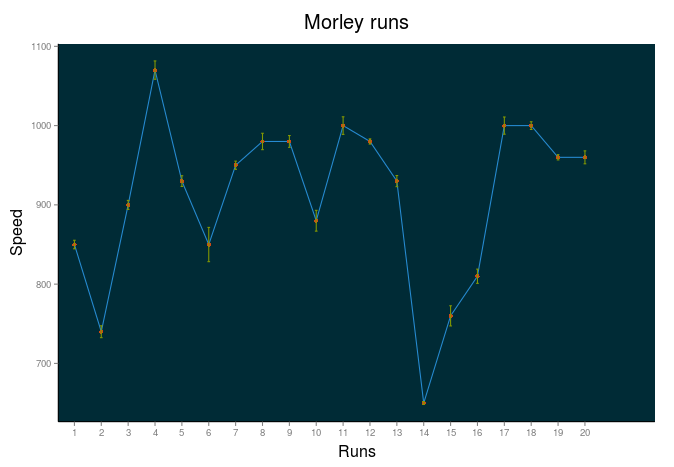
\includegraphics[scale=0.5]{images/error_bars}
 \caption*{Plot with error bars}
\end{figure}

\section{Barplots}
If, instead, we want to have a barplot thereof, just
replace \texttt{geom\_line} (\texttt{geom\_point} respectively)
with

\begin{verbatim}
p <- p + geom_bar(aes(y=Speed),stat='identity', width=.7,
         fill='#657b83', color= '#6c71c4')
\end{verbatim}
\begin{figure}[htbp]
 \centering
 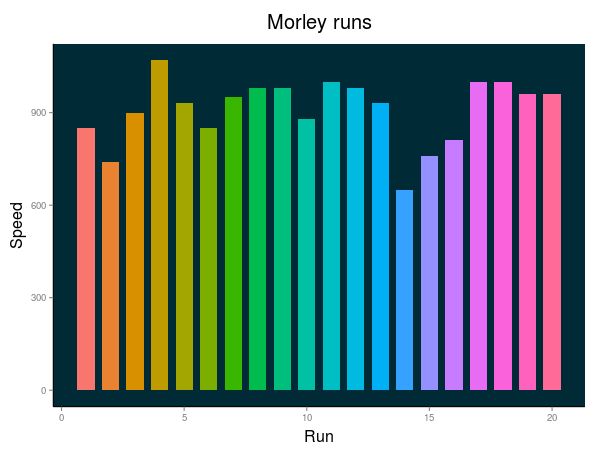
\includegraphics[scale=0.5]{images/barplot}
 \caption*{Barplot}
\end{figure}
                  
How about we unfold the bars in polar coordinates
instead?

\texttt{p <- p + coord\_polar()}

\begin{comment}
\begin{figure}[htbp]
 \centering
 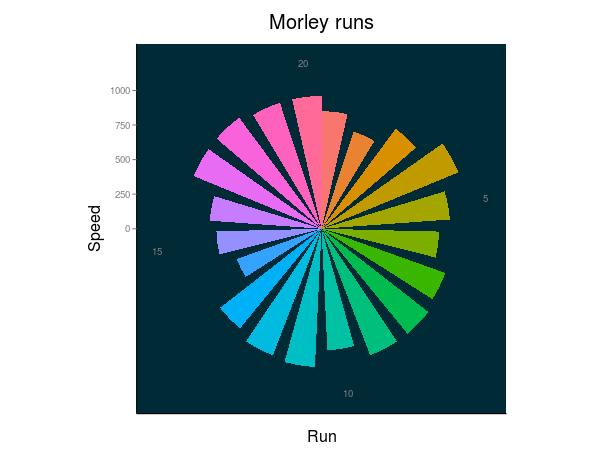
\includegraphics[scale=0.35]{images/polar}
 \caption*{Barplot in polar coordinates}
\end{figure}
\end{comment}

\section{Boxplots}
A boxplot is obtained as follows (\texttt{theme} is kept as before):
\begin{verbatim}
p <- ggplot(morley, aes(x=2, y=morley$Speed))
p <- p + geom_boxplot(outlier.colour = "blue", fill="grey85") 
p <- p + labs(title = "Morley speeds")
p <- p + labs(y = "Speed")
p <- p + labs(x = "")
show(p)
\end{verbatim}
where the values of the $x$ axis is irrelevant. Additional options
can be included with
\begin{verbatim}
p <- p + geom_boxplot(notch = TRUE) 
p <- p + geom_jitter() 
p <- p + geom_hline(aes(yintercept=mean(morley$Speed)), 
	 colour="sienna")
\end{verbatim}

\begin{figure}[htbp]
 \centering
 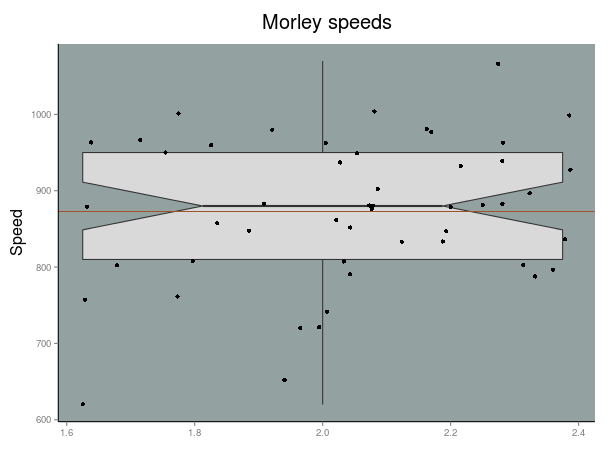
\includegraphics[scale = .50]{images/jitter}
 \caption*{Boxplot with jitters and notches}
\end{figure}

\section{Data grouped by}
Should we have data belonging to different 
groups, it would be convenient to represent
each one of them with different colours, lines
and bars. Here is how:
\begin{verbatim}
library(data.table)
iris   <- data.table(iris)
groups <- iris[, .(length = mean(Sepal.Length)), 
	      by = c("Species", "Sepal.Width")]

p <- ggplot(groups, aes(x=Sepal.Width, y=length, 
		   group = Species, colour= Species))
p <- p + theme(panel.grid.major = element_blank(), 
               panel.grid.minor = element_blank(),
               panel.background = element_rect(fill = '#002b36'),
               axis.line = element_line(colour = "black"),
               legend.text=element_text(size=16),
               legend.title=element_blank(),
               axis.title.x = element_text(vjust=0, size=16),
               axis.title.y = element_text(vjust=1, size=16),
               plot.title   = element_text(vjust=1.5, size=20)) 
p <- p + geom_point()
p <- p + geom_line() 
p <- p + scale_colour_discrete()
p <- p + labs(title = "Iris species")
p <- p + labs(x = "Sepal width")
p <- p + labs(y = "Sepal length")
show(p)      
\end{verbatim}
\begin{figure}[htbp]
 \centering
 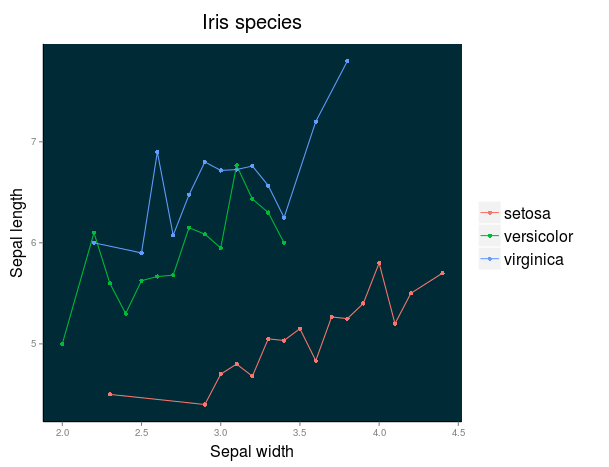
\includegraphics[scale = .65]{images/grouped_colours}
 \caption*{Data grouped by distinguished by colours}
\end{figure}

Equivalently with barplots
\begin{verbatim}
iris <- data.table(iris)
iris$Sepal.Width <- round(iris$Sepal.Width)
groups <- iris[, .(length = mean(Sepal.Length)), 
		  by = c("Species", "Sepal.Width")]


p <- ggplot(groups, aes(x=Sepal.Width, y=length))
p <- p + theme(panel.grid.major = element_blank(), 
               panel.grid.minor = element_blank(),
               panel.background = element_rect(fill = '#002b36'),
               axis.line = element_line(colour = "black"),
               legend.text=element_text(size=16),
               legend.title=element_blank(),
               axis.title.x = element_text(vjust=0, size=16),
               axis.title.y = element_text(vjust=1, size=16),
               plot.title   = element_text(vjust=1.5, size=20)) 
p <- p + geom_bar(aes(fill=Species), width = 0.8, 
                  position = "dodge", stat = "identity")
p <- p + scale_colour_discrete()
p <- p + labs(title = "Iris species")
p <- p + labs(x = "Sepal width")
p <- p + labs(y = "Sepal length")
show(p)
\end{verbatim}
\begin{figure}[htbp]
 \centering
 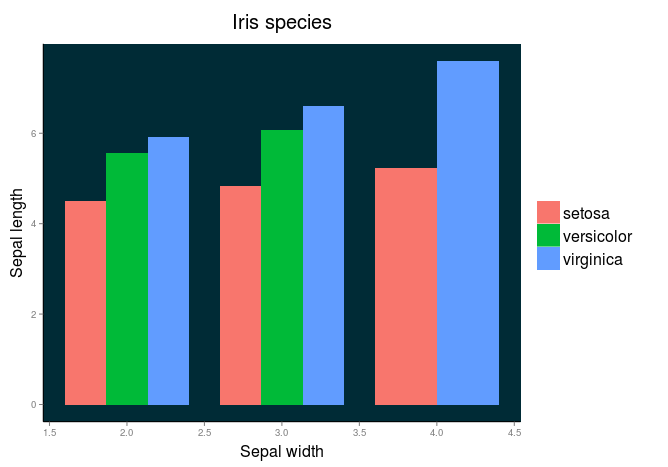
\includegraphics[scale = .5]{images/grouped_barplot}
 \caption*{Barplot of data grouped by}
\end{figure}

The option \texttt{position = "dodge"}
ensures that the bars lie by one other. Taking 
that off would make a stacked barplot instead.
Adding the option \texttt{faced\_grid} allows to move 
different groups to different windows of the graph
\texttt{p <- p + facet\_grid(Species \~ .)}
\begin{figure}[htbp]
 \centering
 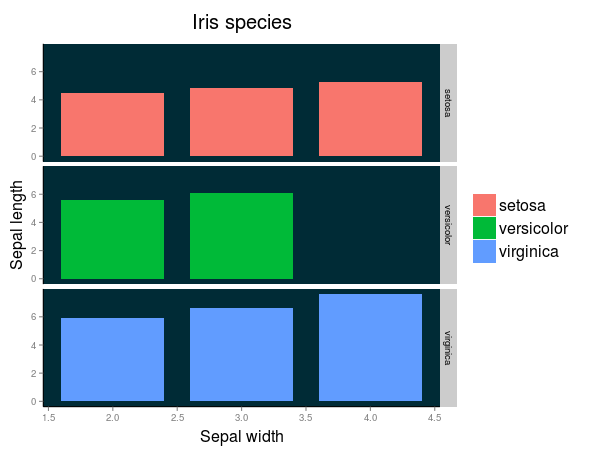
\includegraphics[scale=0.6]{images/facet_grid}
 \caption*{Barplots in different windows}
\end{figure}

\section{Plotting functions}
In order to plot several functions on
the same graph
\begin{verbatim}
p <- ggplot(data.frame(x = c(-5, 5)), aes(x))  
p <- p + stat_function(fun = dnorm, colour = "#2aa198")
p <- p + stat_function(fun = function(x) 2*dnorm(x^2-1), 
		      colour = "#268bd2")
p <- p + theme(panel.grid.major = element_blank(), 
               panel.grid.minor = element_blank(),
               panel.background = element_rect(fill = '#002b36'),
               axis.line = element_line(colour = "black"),
               legend.text=element_text(size=16),
               legend.title=element_blank(),
               axis.title.x = element_text(vjust=0, size=16),
               axis.title.y = element_text(vjust=1, size=16),
               plot.title   = element_text(vjust=1.5, size=20)) 
show(p)
\end{verbatim}
\begin{figure}[htbp]
 \centering
 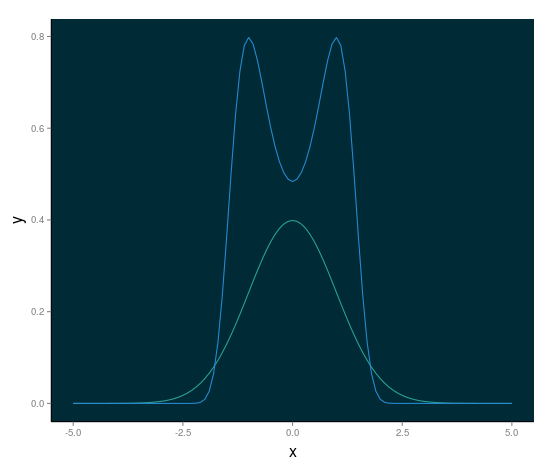
\includegraphics[scale = .45]{images/functions}
 \caption*{Plot of more than one function}
\end{figure}

\section{Histograms}
\texttt{geom\_histogram} does the job. The values 
have to nevertheless be made into a data table 
format, that has to be invoked as first argument
of \texttt{ggplot}
\begin{verbatim}
dt <- data.table(values = rlnorm(50))

p <- ggplot(dt, aes(x=values))
p <- p + theme(panel.grid.major = element_blank(), 
               panel.grid.minor = element_blank(),
               panel.background = element_rect(fill = '#002b36'),
               axis.line = element_line(colour = "black"),
               legend.text=element_text(size=16),
               legend.title=element_blank(),
               axis.title.x = element_text(vjust=0, size=16),
               axis.title.y = element_text(vjust=1, size=16),
               plot.title   = element_text(vjust=1.5, size=20)) 
p <- p + geom_histogram(aes(y=..density.., fill = ..density..), 
                        colour="#002b36", binwidth = 0.3)
p <- p + geom_density(color = "#657b83")
# the below is to manually set the gradient
# p <- p + scale_fill_gradient(low = "red", high = "green")
p <- p + labs(title = "Histogram of normal samples")
show(p) 
\end{verbatim}
\begin{figure}[htbp]
 \centering
 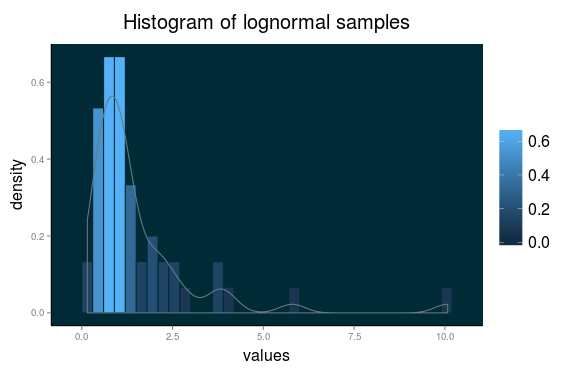
\includegraphics[scale = .45]{images/histogram}
 \caption*{Histogram}
\end{figure}

\section{Tiles}
\texttt{install.packages(scale)}\\
\texttt{library(scale)}
\bigskip 

A powerful visualisation method for many variables
at a time is provided by \texttt{geom\_tile}, where different
values of each variable are represented by different tiles
filled on gradient according to the value: the set 
of data must be molten first and then the variables values
have to be scaled between $\mathopen[0,1\mathclose]$ so 
that one can assign standard gradient fillings. The
example below clarifies the issue:
\begin{verbatim}
cars          <- data.table(mtcars)
cars$carnames <- rownames(mtcars)
cars.molten   <- melt(cars)

R: cars.molten <- data.table(cars.molten)
R: cars.molten[sample(.N,5)]

              carnames variable value
1:            Merc 230     qsec 22.90
2:         Honda Civic       am  1.00
3:           Merc 240D     drat  3.69
4: Lincoln Continental      mpg 10.40
5:          Merc 450SL       am  0.00
\end{verbatim}
We now make use of the \texttt{rescale} function
in the \texttt{scale} package as:
\begin{verbatim}
cars.molten <- ddply(cars.molten, .(variable), transform,
                rescale = rescale(value)) 
R: cars.molten <- data.table(cars.molten)
R: cars.molten[sample(.N,5)]

              carnames variable value   rescale
1:          Camaro Z28      mpg  13.3 0.1234043
2:          Merc 450SE      mpg  16.4 0.2553191
3:          Camaro Z28     disp 350.0 0.6956847
4: Lincoln Continental       hp 215.0 0.5759717
5:           Merc 280C     qsec  18.9 0.5238095

p <- ggplot(cars.molten, aes(x=variable, y = carnames, 
                                      fill = rescale))
p <- p + theme(panel.grid.major = element_blank(), 
               panel.grid.minor = element_blank(),
               panel.background = element_rect(fill 
                                            = '#002b36'),
               axis.line = element_line(colour = "black"),
               legend.text=element_text(size=16),
               legend.title=element_blank(),
               axis.title.x = element_text(vjust=0, 
                                     size=16),
               axis.title.y = element_text(vjust=1, size=16),
               plot.title   = element_text(vjust=1.5, size=20)) 
p <- p + geom_tile(colour = "#002b36")
p <- p + scale_fill_gradient(low = "steelblue", 
                             high = "#002b36")
p <- p + labs(x = "")
show(p)
\end{verbatim}
Tiled results are shown in the plot below, whit the 
row names arranged on the $y$ axis and the variables 
displayed horizontally instead.
\begin{figure}[htbp]
 \centering
 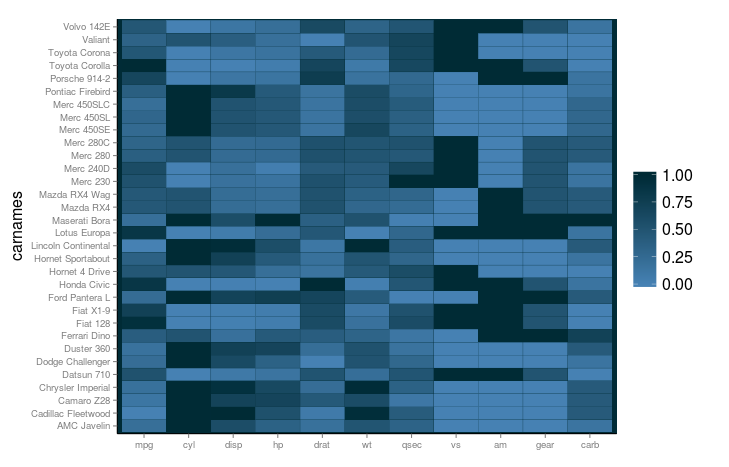
\includegraphics[scale=0.5]{images/tiles}
 \caption*{Tiled heatmap}
\end{figure}
%************************************************
\chapter{The \pkgname{reshape2} package}\label{sec: reshape2}
%************************************************
\texttt{install.packages(`reshape2')}\\
\texttt{library(`reshape2')}
\bigskip 

The library \texttt{reshape} is mainly based on 
two functions: \texttt{dcast} and \texttt{melt} to
reshape the data. The former transforms a \emph{long}
data frame into a \emph{wide} one and the latter
does viceversa.
\bigskip

A long data frame is such when one (or more variables)
are arranged as row entries rather than columns instead.
If so, those variables can be re-arranged back into 
columns whose values will be function of other choses ones.
For instance, given the \texttt{quarks} data table, we can
calculate the mode (making use of the function in 
\ref{sec: functions}) for each quark in each laboratory.
The syntax is 
\texttt{dcast(dt, col1 + ... + colN \~ variable, fun.aggregate = fun)} 
\begin{verbatim}
R: dcast(quarks, lab ~flavour,  fun.aggregate = mode)
   
   Using S_z as value column.  Use the value argument 
   to cast to override this choice lab bottom charme 
   down strange  top   up

   lab bottom charme down strange  top   up
1   A   <NA>    1/2  1/2     1/2 -1/2 <NA>
2   B    1/2    1/2  1/2     1/2  1/2 <NA>
3   C    1/2    1/2  1/2     1/2  1/2  1/2
4   D    1/2    1/2  1/2    -1/2  1/2  1/2
5   E    1/2   -1/2 -1/2    -1/2  1/2 -1/2
6   F    1/2    1/2 -1/2    -1/2 <NA> -1/2
\end{verbatim}

\texttt{dcast} does not work when more than a value is
present per variable: a function must be provided
(\texttt{mode} in the example above). To illustrate
the converse behaviour we are using the in-built 
data set \texttt{airquality}.
\begin{verbatim}
R: head(airquality)

  Ozone Solar.R Wind Temp Month Day
1    41     190  7.4   67     5   1
2    36     118  8.0   72     5   2
3    12     149 12.6   74     5   3
4    18     313 11.5   62     5   4
5    NA      NA 14.3   56     5   5
6    28      NA 14.9   66     5   6
\end{verbatim}
One may want to make some of the columns row
entries instead, keeping just some others as
fixed. For instance we fix ``Month'' and 
``Day'' and melt the rest accordingly
\begin{verbatim}
melt(airquality, id.vars = c("Month", "Day")) 
 
R: head(melt(airquality, id.vars = c("Month", "Day")))
  Month Day variable value
1     5   1    Ozone    41
2     5   2    Ozone    36
3     5   3    Ozone    12
4     5   4    Ozone    18
5     5   5    Ozone    NA
6     5   6    Ozone    28

R: tail(melt(airquality, id.vars = c("Month", "Day")))
    Month Day variable value
607     9  25     Temp    63
608     9  26     Temp    70
609     9  27     Temp    77
610     9  28     Temp    75
611     9  29     Temp    76
612     9  30     Temp    68

R: data.table(melt(airquality, id.vars = 
                     c("Month", "Day")))[sample(.N,5)]
   Month Day variable value
1:     9  14     Wind  10.9
2:     7  13  Solar.R 175.0
3:     5  18     Temp  57.0
4:     5   7    Ozone  23.0
5:     8  21     Temp  77.0
\end{verbatim}
Molten data are meant to be used to plot
statistics in groups, especially histograms
for each molten variable. The below is an 
example:
\begin{verbatim}

R: iris.molten <- melt(iris, id.vars = "Species")
R: iris.molten <- data.table(iris.molten)
R: iris.molten[sample(.N,5)]

      Species     variable value
1:  virginica  Sepal.Width   2.9
2: versicolor  Sepal.Width   2.5
3:  virginica  Petal.Width   2.0
4: versicolor Sepal.Length   6.1
5:     setosa Sepal.Length   4.5

p <- ggplot(iris.molten, aes(x=value, fill = Species))
p <- p + theme(panel.grid.major = element_blank(), 
               panel.grid.minor = element_blank(),
               panel.background = element_rect(fill 
                                               = '#002b36'),
               axis.line = element_line(colour = "black"),
               legend.text=element_text(size=16),
               legend.title=element_blank(),
               axis.title.x = element_text(vjust=0, size=16),
               axis.title.y = element_text(vjust=1, size=16),
               plot.title   = element_text(vjust=1.5, size=20)) 
p <- p + geom_histogram(aes(y = ..density..), position = "dodge",
                        binwidth = 0.25, colour = "#002b36")
p <- p + facet_wrap( ~ variable, scales="free")
p <- p + guides(fill = guide_legend(override.aes = 
                                        list(colour = NULL)))
p <- p + labs(title = "Iris histograms")
p <- p + labs(x = "variable")
p <- p + labs(y = "density")
show(p)
\end{verbatim}
\begin{figure}[htbp]
 \centering
 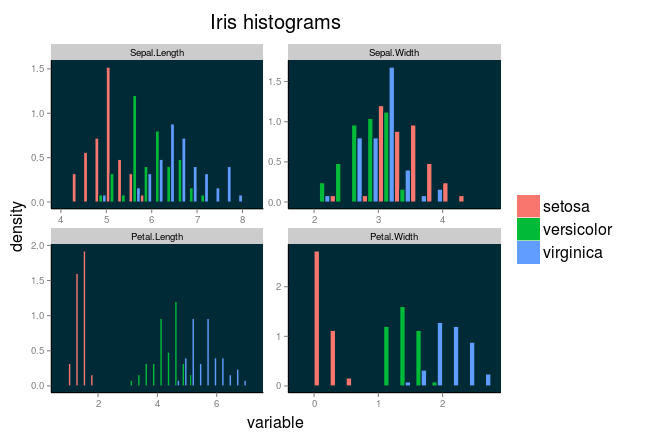
\includegraphics[scale = 0.5]{images/facet_wrap}
 \caption*{Molten data set histograms}
\end{figure}
Obviously, if we cast the molten data table 
back, we obtain the data we started with,
by definition.

\begin{verbatim}
R: dcast(melt(airquality, id.vars = c("Month", "Day")), 
        Month + Day ~ variable)
        
  Month Day Ozone Solar.R Wind Temp
1     5   1    41     190  7.4   67
2     5   2    36     118  8.0   72
3     5   3    12     149 12.6   74
4     5   4    18     313 11.5   62
5     5   5    NA      NA 14.3   56
6     5   6    28      NA 14.9   66        
\end{verbatim}





%************************************************
\chapter{Data clustering}\label{sec: clusters}
%************************************************

\section*{Hierarchical clustering and dendograms}
Hierarchical clustering pairwise groups 
variables according to the minimum distances,
and so on and so forth until the entire data 
set is reconstructed and tree shaped. Distances
between points can be calculated using any
distance $d(x,y)$ via
\texttt{dist(df, method = <method>)}, the data frame
containing the rows as points whose distances one
wants to calculate. 
\medskip 

As an example we can hierarchically cluster a subset
of the \texttt{mtcars} data starting from calculating 
its euclidean distances among different rows (which, 
in turn, represent the different points that we want
to cluster)
\begin{verbatim}
distances <- dist(iris, method = "euclidean")
dendog    <- hclust(distances, method = "ave") 
\end{verbatim}
The function \texttt{hclust} pairwise couples the points
according to the minimum distance, going up in pairs until
the whole data set is exhausted.
\bigskip
The dendogram can be plotted making use of the 
following packages:\\
\texttt{library("ggplot2")}\\
\texttt{install.packages("ggdendro")}\\
\texttt{library("ggdendro")}
\bigskip 

\begin{verbatim}
# dendro_data extracts the dendogram 
# objects numerical data
dendog    <- dendro_data(dendog, type = "rectangle")

p <- ggplot(segment(dendog)) 
p <- p + theme(panel.grid.major = element_blank(), 
               panel.grid.minor = element_blank(),
               panel.background = element_rect(fill 
                                               = '#002b36'),
               axis.line = element_line(colour = "black"),
               legend.text=element_text(size=16),
               legend.title=element_blank(),
               axis.title.x = element_text(vjust=0, size=16),
               axis.title.y = element_text(vjust=1, size=16),
               plot.title   = element_text(vjust=1.5, size=20))
p <- p + geom_segment(aes(x = x, y = y, 
                      xend = xend, yend = yend),
                      colour = "white", alpha = 0.7)
p <- p + geom_text(data = label(dendog), colour = "white", 
                   aes(x = x+0.5, y = -5, label = label),
                   vjust = 1.2, hjust = 0)
p <- p + coord_flip()
p <- p + scale_y_reverse(expand = c(0.2, 0))
p <- p + labs(x = "cars")
p <- p + labs(y = "")
show(p)
\end{verbatim}
\begin{figure}[htbp]
 \centering
 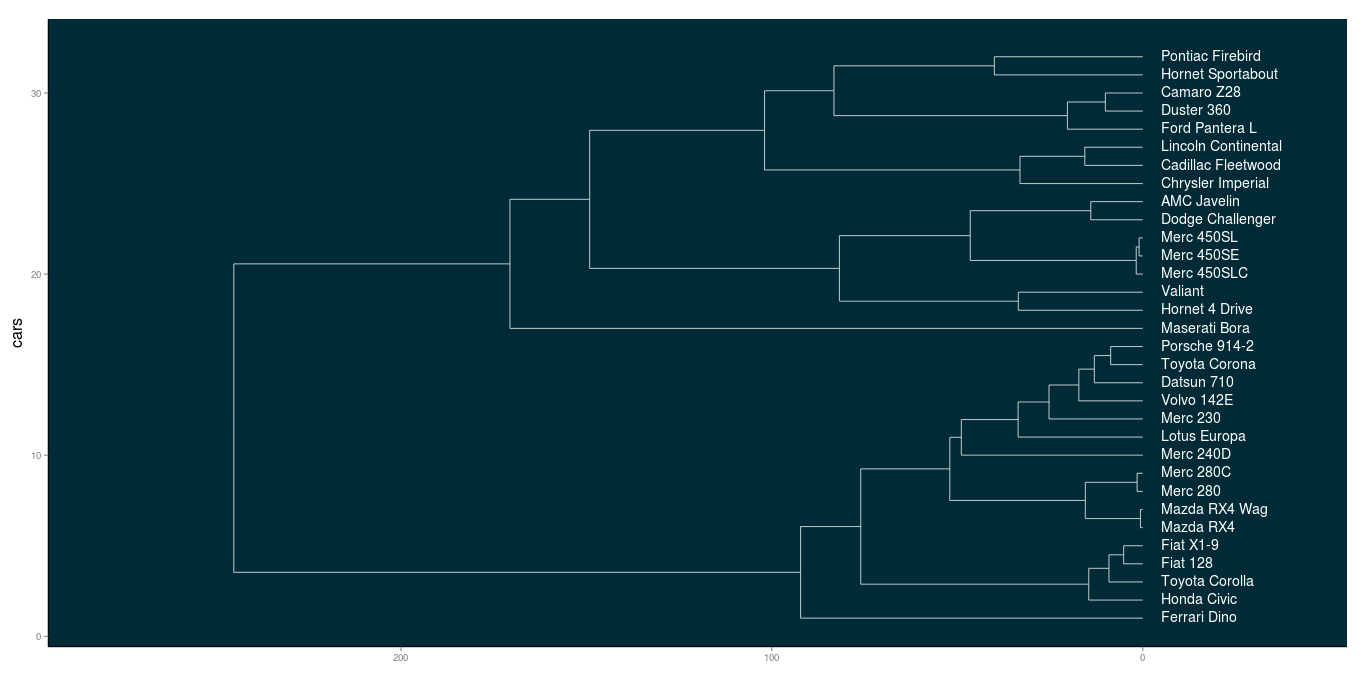
\includegraphics[scale=0.25]{images/dendo}
 \caption*{Hierarchical clustering dendogram}
\end{figure}

\section{$k$-means clustering}
$k$-means clustering groups the data
in clusters according to the shortest
distances to the centres of the cluster,
whose number may be manually set. How to
properly calculate the correct number
of clusters and their centres will not 
be investigated here and we refer the 
reader to standard literature for that.
\bigskip

\texttt{kmeans} needs a set of data whose 
rows represent different point, whose 
coordinates are in turn given as column
entries; all the provided values must be
in numerical format. Different methods to calculate
the clusters can be specified as additional
arguments and options parameters.
\begin{verbatim}
# storing the names 
names <- iris[,5]
iris  <- iris[-5]

cluster <- kmeans(iris, centers = 3)

# coordinates of the centres
R: cluster$centers

  Sepal.Length Sepal.Width Petal.Length Petal.Width
1     5.006000    3.428000     1.462000    0.246000
2     5.901613    2.748387     4.393548    1.433871
3     6.850000    3.073684     5.742105    2.071053

# dimensions of the clusters
R: cluster$size

[1] 50 62 38

# each labelled row belongs to the specified cluster
R: cluster$cluster

  [1] 1 1 1 1 1 1 1 1 1 1 1 1 1 1 1 1 1 1 1 1...
 [38] 1 1 1 1 1 1 1 1 1 1 1 1 1 2 2 3 2 2 2 2...
 [75] 2 2 2 3 2 2 2 2 2 2 2 2 2 2 2 2 2 2 2 2...
[112] 3 3 2 2 3 3 3 3 2 3 2 3 2 3 3 2 2 3 3 3...
[149] 3 2
\end{verbatim}
Additional information can be gained investigating
the outcome values of the function \texttt{kmeans}.
However, row names can be placed back against the 
clusters labels as
\begin{verbatim}
R: table(names, cluster$cluster)
            
names         1  2  3
  setosa     50  0  0
  versicolor  0 48  2
  virginica   0 14 36
\end{verbatim}
\medskip 

Clustering can be made use of to spot 
possible outliers in the set of data, 
as those point having the furthest distances
from any of the clusters centres.
\begin{verbatim}
centres   <- cluster$centers[cluster$cluster,]
distances <- sqrt(rowSums((iris-centres)^2))

outliers  <- head(iris[order(distances, decreasing = TRUE),])

R: outliers

    Sepal.Length Sepal.Width Petal.Length Petal.Width
99           5.1         2.5          3.0         1.1
58           4.9         2.4          3.3         1.0
94           5.0         2.3          3.3         1.0
61           5.0         2.0          3.5         1.0
119          7.7         2.6          6.9         2.3
118          7.7         3.8          6.7         2.2
\end{verbatim}
The above can be made into a function, such that, given 
a data set, one can return the first $M$ outliers once 
a clustering around $N$ groups has been performed:
\begin{verbatim}
outlier.by.clustering <- function(df,N,M){
    cluster   <- kmeans(df, centers = N)
    centres   <- cluster$centers[cluster$cluster,]
    distances <- sqrt(rowSums((df-centres)^2))
    outliers  <- head(df[order(distances, 
                      decreasing = TRUE),],M)
    return(outliers)
}

R: outlier.by.clustering(iris,3,5)

    Sepal.Length Sepal.Width Petal.Length Petal.Width
99           5.1         2.5          3.0         1.1
58           4.9         2.4          3.3         1.0
94           5.0         2.3          3.3         1.0
61           5.0         2.0          3.5         1.0
119          7.7         2.6          6.9         2.3
\end{verbatim}




%************************************************
\chapter{Hypotheses tests}\label{sec: tests}
%************************************************
\section{Normality tests and qq-plots}
Hypotheses tests \emph{against} the normal 
Gau\ss ian distribution can be performed 
starting with the \texttt{shapiro.test(values)}.
The sample size affects
the results of the normality test:
\begin{verbatim}
set.seed(1)
x <- rlnorm(20, 0 ,.4)
y <- rlnorm(100, 0, .4)

R: shapiro.test(x)
R: shapiro.test(y)

	        Shapiro-Wilk normality test

data:  x                      | data: y
W = 0.98049, p-value = 0.9403 | W = 0.91864, p-value = 1.193e-05
\end{verbatim}
In small sample sizes, even big departures from
normality are not detected. QQ-plots help us to
represent deviations from normality, as in the
example below:
\begin{verbatim}
R: mtcars[, .(p.value = shapiro.test(mpg)[2]), 
             by = "cyl"]

   cyl   p.value
1:   6 0.3251776
2:   4 0.2605931
3:   8 0.3228563

p <- ggplot(mtcars, aes(sample = mpg, colour = factor(cyl)))
p <- p + theme(panel.grid.major = element_blank(), 
               panel.grid.minor = element_blank(),
               panel.background = element_rect(fill = '#002b36'),
               axis.line = element_line(colour = "black"),
               legend.text=element_text(size=16),
               legend.title=element_blank(),
               axis.title.x = element_text(vjust=0, size=16),
               axis.title.y = element_text(vjust=1, size=16),
               plot.title   = element_text(vjust=1.5, size=20)) 
p <- p + stat_qq()
show(p)
\end{verbatim}
\begin{figure}[htbp]
 \centering
 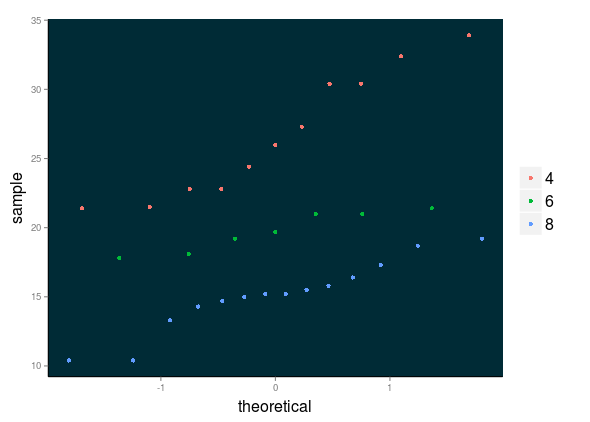
\includegraphics[scale=.6]{images/qqplots}
 \caption*{QQ-plot for data grouped by}
\end{figure}
Let us define a function that shows the rejection tests 
against the normal distribution for a set of 
grouped data, once an initial $p$-value is set.
\begin{verbatim}
shapiro.p.value <- function(my.column) {
    my.p.value <- '0.05'
    if(shapiro.test(my.column)[2] < my.p.value){
        return("rejected")
    } else {
        return("not rejected")
    }
} 
 
R: iris[, lapply(.SD, shapiro.p.value), by = Species]

      Species Sepal.Length  Sepal.Width Petal.Length  Petal.Width
1:     setosa not rejected not rejected not rejected not rejected
2: versicolor not rejected not rejected not rejected     rejected
3:  virginica not rejected not rejected not rejected not rejected
\end{verbatim}

\section{t-tests}
Student's t-test can be performed againts two 
sets of values to have the null hypothesis that their
means and variances to be the same, under the underlying 
assumption for both samples to come from a normal distribution.
If this were true, then the t-test statistic  
$t=\frac{(\bar{x}-\mu_0)}{(s/\sqrt{n})(\sigma/\sqrt{n})}$ would follow
a Student's t-distribution with $n_1 + n_2 -2$ degrees
of freedom, $n_1, n_2$ being the samples sizes.
For additional references, please see\footnote{ 
\url{http://statistics.berkeley.edu/computing/r-t-tests}
}
\medskip 

As an example we consider two normal samples and test 
the $t$-statistic obtained after $N$ t-tests. Given 
two sets of data $x, y$ then
\begin{verbatim}
set.seed(1)
tt <- t.test(rnorm(10), rnorm(10))

R: tt

	Welch Two Sample t-test

data:  rnorm(10) and rnorm(10)
t = -0.27858, df = 16.469, p-value = 0.784
alternative hypothesis: true difference 
in means is not equal to 0
95 percent confidence interval:
 -1.0022169  0.7689325
sample estimates:
mean of x mean of y 
0.1322028 0.2488450 

R: names(tt)
[1] "statistic"   "parameter"   "p.value"     "conf.int"       
[6] "estimate" "null.value"  "alternative" "method"      
[10] "data.name"
\end{verbatim}
where we are interested in the \texttt{statistic} parameter.
Therefore
\begin{verbatim}
    N <- 10000
tstat <- replicate(N, t.test(rnorm(10),rnorm(10))$statistic)

points <- seq(range(tstat)[1], range(tstat)[2], length=100)

# theoretical values of the t-distribution
theory <- dt(points, df = 10+10-2)  
# density values of the obtained t-statistics.
num    <- density(tstat, n=100)$y

data   <- data.table(points = points, theory = theory,
                     num = num)

p <- ggplot(data, aes(x=points))
p <- p + theme(panel.grid.major = element_blank(), 
               panel.grid.minor = element_blank(),
               panel.background = element_rect(fill = '#002b36'),
               axis.line = element_line(colour = "black"),
               legend.text=element_text(size=16),
               legend.title=element_blank(),
               axis.title.x = element_text(vjust=0, size=16),
               axis.title.y = element_text(vjust=1, size=16),
               plot.title   = element_text(vjust=1.5, size=20)) 
p <- p + geom_line(aes(y=theory, colour = "theory"))
p <- p + geom_line(aes(y=num, colour = "data"))
p <- p + scale_colour_manual(values=c("#2aa198","#268bd2"))
p <- p + labs(title = "t-test statistics")
p <- p + labs(y = "densities")
show(p)  
\end{verbatim}
\begin{figure}[htbp]
 \centering
 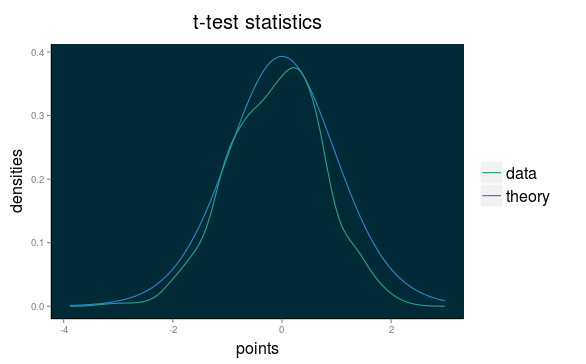
\includegraphics[scale=.6]{images/t_test}
 \caption*{$t$-test statistics densities}
\end{figure}
Another way to compare two densities is with 
a quantile-quantile plot. In this type of plot 
the quantiles of two samples are calculated at 
a variety of points in the range 
$\mathopen[0,1\mathopen]$, 
and then are plotted against each other. If the 
two samples came from the same distribution with 
the same parameters, we would see a straight line through 
the origin with unit slope; in other words, we are 
testing to see if various quantiles of the data are 
identical in the two samples. If the two samples came 
from similar distributions, but their parameters were 
different, we would still see a straight line, 
but not through the origin.
\bigskip

We will get \texttt{qqplot} to perform the necessary
calculations and then use \texttt{ggplot2} to 
display them.
\begin{verbatim}
x <- rnorm(100)
y <- rnorm(100)

dt <- as.data.table(qqplot(x, y, plot.it=FALSE))

p <- ggplot(dt)
p <- p + theme(panel.grid.major = element_blank(), 
               panel.grid.minor = element_blank(),
               panel.background = element_rect(fill = '#002b36'),
               axis.line = element_line(colour = "black"),
               legend.text=element_text(size=16),
               legend.title=element_blank(),
               axis.title.x = element_text(vjust=0, size=16),
               axis.title.y = element_text(vjust=1, size=16),
               plot.title   = element_text(vjust=1.5, size=20)) 
p <- p + geom_point(aes(x=x, y=y, colour = "QQ-plot"))
p <- p + geom_abline(aes(colour="ideal"), 
                     intercept = 0, slope = 1)
p <- p + scale_colour_manual(values=c("#2aa198","#268bd2"))
p <- p + labs(title = "t-test statistics")
p <- p + labs(y = "densities")
show(p)  
\end{verbatim}
\begin{figure}[htbp]
 \centering
 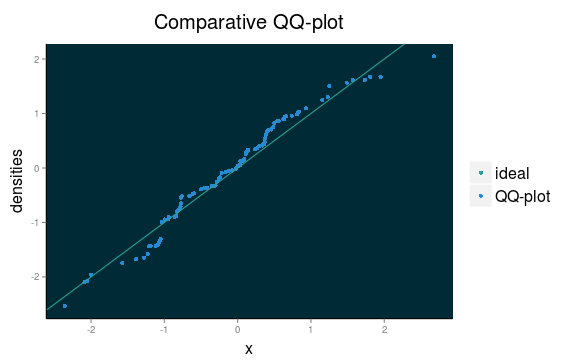
\includegraphics[scale=.6]{images/two_distr_qq}
 \caption*{QQ-plots to compare two distributions}
\end{figure}
Equivalently, if the null hypothesis were true,
namely if the two sets of data came from the 
same distribution, the $p$-value distribution
would be uniform. Doing so on the above analysis
we have
\begin{verbatim}
     N <- 10000
tpstat <- replicate(N,t.test(rnorm(10),rnorm(10))$p.value)
points <- seq(range(tpstat)[1], range(tpstat)[2], length=100)
# density values of the obtained p-values.
num    <- density(tpstat, n=100)$y
data   <- data.table(points = points, num = num)
\end{verbatim}
\begin{figure}[htbp]
 \centering
 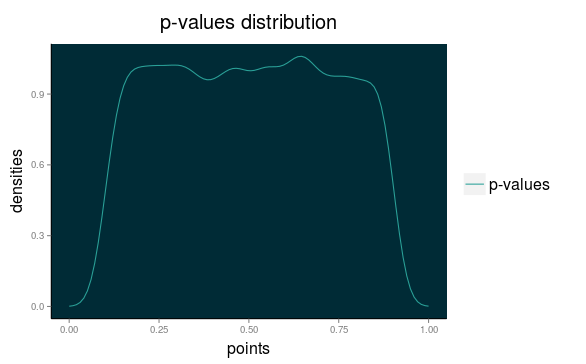
\includegraphics[scale=.6]{images/p_value_distr}
 \caption*{$p$-value uniform distribution}
\end{figure}

\section{Kruskal-Wallist test}
A collection of data samples are independent 
if they come from unrelated populations and 
the samples do not affect each other. Using the 
Kruskal-Wallis Test, we can decide whether the 
population distributions are identical without 
assuming them to follow the normal distribution.
\bigskip 

As a matter of example we can test 
whether the petal width in the \texttt{iris}
data set come from different distributions,
according the species. The null hypothesis 
is that they are identical populations:
\begin{verbatim}
R: kruskal.test(Petal.Width ~ Species, data = iris)

	Kruskal-Wallis rank sum test

data:  Petal.Width by Species
Kruskal-Wallis chi-squared = 131.19, df = 2, p-value < 2.2e-16
\end{verbatim}
It is therefore very \emph{unlikely} ($p$-value $<0.05$) 
the populations are identical.

\section{Dunn's test}

After having found out that a certain sets of data
come from dissimilar distributions, it is
possible to pairwise compare them to realise
which specific couplings disturb the entire set.
The above is obtained by means of the Dunn's test.
\begin{verbatim}
R: dunn.test(iris$Sepal.Width, g = iris$Species)

        Kruskal-Wallis rank sum test

data: x and group
Kruskal-Wallis chi-squared = 63.5711, df = 2, p-value = 0


              Comparison of x by group                            
                (No adjustment)                                
Col Mean-|
Row Mean |     setosa   versicol
---------+----------------------
versicol |   7.787706
         |     0.0000
         |
virginic |   5.374419  -2.413287
         |     0.0000     0.0079

R: dunn.test(iris$Sepal.Width, g = iris$Species)$P

[1] 3.411812e-15 3.841494e-08 7.904669e-03
\end{verbatim}
The pairwise $p$-values are smaller than any 
threshold, hence all three groups come from
three dissimilar populations.





%************************************************
\chapter{Date and time formats: lubridate}\label{sec: time}
%************************************************
The function \texttt{as.Date} converts the most
date formats given to \emph{input} them 
into the rules of the ISO-8601 
international standard, which expresses the dates
as year-month-day. The format to be converted 
must correspond to the introduced date format:
\begin{verbatim}
date1 <- as.Date("19/02/87", format = "%d/%m/%y")
date2 <- as.Date("04-06-15", format = "%d-%m-%y")

R: date1
[1] "1987-02-19"

R: date1 > date2
[1] FALSE

R: year(date1)
[1] 1987

R: week(date1)
[1] 8
\end{verbatim}

Different placeholders after the percentage sign $\%$
correspond to different date formats. A full list is
available here\footnote{
\url{https://stat.ethz.ch/R-manual/R-patched/library/base/html/strptime.html}}.
Also, the function \texttt{strptime} converts between character 
representations and objects obigf classes "POSIXlt" 
and "POSIXct" representing calendar dates and times;
consequently, it is used to \emph{output} a given date in a 
different desired time format or representation.
\medskip 
The functions \texttt{as.POSIXct} and \texttt{as.POSIXlt}
give representation in the central (local, respectively)
time stamp format as
\begin{verbatim}
R: as.POSIXct(Sys.Date())
[1] "2015-10-17 02:00:00 CEST"

R: as.POSIXlt(Sys.Date())
[1] "2015-10-17 UTC" 
\end{verbatim}
\bigskip

The package \texttt{lubridate} simplifies the date and
time arithmetics as
\begin{verbatim}
install.package(lubridate)
library(lubridate)

R: date1  + weeks(5)
[1] "1987-03-26"

R: date1 - years(2)
[1] "1985-02-19"
\end{verbatim}
Also notice the additional functions giving back
precise information on the weekday and position in
the year as \texttt{ymd\_hms} or 
\begin{verbatim}
R: wday(Sys.Date())
[1] 7

R: wday(Sys.Date(), label = TRUE)
[1] Sat 
\end{verbatim}
and the function \texttt{isoweek}
\begin{verbatim}
date1 <- as.Date("2014-12-31")

R: isoweek(date1)
[1] 1
R: week(date1)
[1] 53
\end{verbatim}

%************************************************
\chapter{Writing and reading data}\label{sec: read_write}
%************************************************
Below is an example on how to write out and read 
in data sets. 
\begin{verbatim}
set.seed(10)
mtcars <- data.table(mtcars)
cars   <- mtcars[sample(.N,5), sample(11,4), with = FALSE]

write.table(cars, file = "my_file.csv", sep = "\t", 
            quote = FALSE, append = FALSE, na = "NA", 
            dec = ".", row.names = FALSE)

read_cars <- read.table("my_file.csv", sep = "\t", quote = "",
                        header = TRUE, dec = ".", fill = FALSE, 
                        na.strings = c("NA", "-"), 
                        stringsAsFactors = FALSE)
                        
R: cars                  | R: read_cars

    disp carb gear drat  |    disp carb gear drat
1: 440.0    4    3 3.23  |1: 440.0    4    3 3.23
2: 167.6    4    4 3.92  |2: 167.6    4    4 3.92
3: 275.8    3    3 3.07  |3: 275.8    3    3 3.07
4: 120.1    1    3 3.70  |4: 120.1    1    3 3.70
5: 108.0    1    4 3.85  |5: 108.0    1    4 3.85        
\end{verbatim}
The option \texttt{na.strings = c("NA", "-")} decides
which lines must be interpreted as \texttt{NA}. 
Likewise \texttt{fill = TRUE} allows to skip and 
continue whenever inconsistencies in the data are
present: on the other hand \texttt{fill = FALSE} 
throws an error whenever so (and hence allows 
control on the inconsistent data). To trim leading 
and tailing space from unquoted strings use 
\texttt{strip.white = TRUE}.
\bigskip

The \texttt{data.table} package makes use of 
\texttt{fread} to read data file in, this being
much faster (especially for large sets of data),
while keeping the same syntax.

%************************************************
\chapter{Text manipulation}\label{sec: text}
%************************************************
\texttt{install.package(stringr)}\\
\texttt{library(stringr)}
\bigskip 

Use \texttt{str\_trim} to trim leading and 
tailing white spaces:
\begin{verbatim}
s <- ' Hello, world! '

R: str_trim(s, side = "left") | R: str_trim(s, side = "right")
[1] "Hello, world! "          | [1] " Hello, world!"

R: str_trim(s)                | R: str_trim("\n\nHello, world!\t")
[1] "Hello, world!"           | [1] "Hello, world!"
\end{verbatim}
In order to replace \emph{all} white space (and likewise
any other character) use \texttt{str\_replace\_all}.
\begin{verbatim}
R: str_replace_all(s, fixed(" "), "") 

[1] "Hello,world!"

R: str_replace_all(s, "l", "!")
[1] " He!!o, wor!d! "
\end{verbatim}
The functions \texttt{tolower} and \texttt{toupper}
do the job as named:
\begin{verbatim}
R: tolower(s)         | R: toupper(s)
[1] "hello, world!"   | [1] "HELLO, WORLD!"
\end{verbatim}
Strings can be alphabetically sorted using the 
\texttt{sort} numerical function plus a little manipulation
of the characters. This can be useful when checking
whether a certain number of words having the same number
of characters are anagrams of one other: the standars
procedure is to split their letters and sort them
alphabetically to match them. 
\begin{verbatim}
sort.word <- function(x){
 x <- tolower(x)
 x <- str_replace_all(x, fixed(" "), "")    
 x <- paste(sort(unlist(strsplit(x, ""))), collapse = "") 
 return(x)
}

is.anagram <- function(x,y){
    return(sort.word(x) == sort.word(y))
}

first  <- "Eleven plus Two"
second <- "Twelve plus One"
third  <- "Ten plus three"

R: is.anagram(first, second)    | R: is.anagram(first, third)
[1] TRUE                        | [1] FALSE                        
\end{verbatim}


\renewcommand{\thesection}{A}
%************************************************
\chapter{Special functions}\label{sec: functions}
%************************************************
A collection of useful (non-in-built) functions.
\bigskip

\begin{itemize}
\item[-] \emph{Mode}:
\begin{verbatim}
mode <- function(x) {
	ux <- unique(x)
	ux[which.max(tabulate(match(x, ux)))]
}
	
R: mode(quarks$flavour)
[1] "strange"
\end{verbatim}
	
\item[-]\emph{na2zero}:
\begin{verbatim}
na2zero <- function(x) {
	x[] <- lapply(x,function(x){x[is.na(x)] <- 0; x})
	x
}
\end{verbatim}
	
\item[-]\emph{Cartesian product}
\begin{verbatim}
cross.join <- function(a, b) {
	idx <- expand.grid(seq(length=nrow(a)), 
                           seq(length=nrow(b)))
	cbind(a[idx[,1],], b[idx[,2],])
}
\end{verbatim}
	
 \item[-]\emph{Shapiro $p$-value rejections}
\begin{verbatim}
shapiro.p.value <- function(my.column) {
	my.p.value <- '0.05'
	if(shapiro.test(my.column)[2] < my.p.value){
		return("rejected")
	} else {
		return("not rejected")
	}
}
	
R: iris[, lapply(.SD, shapiro.p.value), by = Species]
      Species Sepal.Length  Sepal.Width Petal.Length   
1:     setosa not rejected not rejected not rejected 
2: versicolor not rejected not rejected not rejected 
3:  virginica not rejected not rejected not rejected 
\end{verbatim}
 \item[-] \emph{Anagrams}
\begin{verbatim}
sort.word <- function(x){
 x <- tolower(x)
 x <- str_replace_all(x, fixed(" "), "")    
 x <- paste(sort(unlist(strsplit(x, ""))), collapse = "") 
 return(x)
}

is.anagram <- function(x,y){
    return(sort.word(x) == sort.word(y))
}

first  <- "Eleven plus Two"
second <- "Twelve plus One"

R: is.anagram(first, second) 
[1] TRUE
\end{verbatim}

 \item[-] \emph{Outliers by clustering}
\begin{verbatim}
outlier.by.clustering <- function(df,N,M){
    cluster   <- kmeans(df, centers = N)
    centres   <- cluster$centers[cluster$cluster,]
    distances <- sqrt(rowSums((df-centres)^2))
    outliers  <- head(df[order(distances, 
                      decreasing = TRUE),],M)
    return(outliers)
}

R: outlier.by.clustering(mtcars[,1:7], 5, 5)

                     mpg cyl disp  hp drat    wt  qsec
Maserati Bora       15.0   8  301 335 3.54 3.570 14.60
Cadillac Fleetwood  10.4   8  472 205 2.93 5.250 17.98
Lincoln Continental 10.4   8  460 215 3.00 5.424 17.82
Hornet Sportabout   18.7   8  360 175 3.15 3.440 17.02
Pontiac Firebird    19.2   8  400 175 3.08 3.845 17.05
\end{verbatim}

\end{itemize}

\begin{comment}
\section{RXKCD}
\texttt{install.packages(RXKCD)}\\
\texttt{library(RXKCD)}
\bigskip

The above fetches comic strips from 
\verb+XKCD+\footnote{
\url{http://xkcd.com/}
}

\texttt{R: getXKCD(which = "random")}
\begin{figure}[!h]
 \centering 
 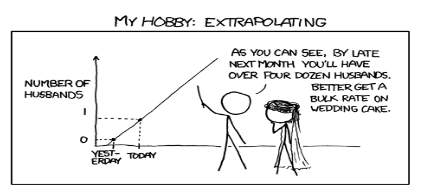
\includegraphics[scale=0.7]{images/xkcd}
 \caption{XKCD strip fetched in \texttt{R}} 
\end{figure}


\section{Colour palette}
I have used the following colour palette
(inspired from ``Solarized''%
\footnote{
\url{http://ethanschoonover.com/solarized}
})
\begin{itemize}
 \item[-] Background: \#002b36
 \item[-] Bars:       \#657b83
 \item[-] Lines:      \#2aa198, \#268bd2
\end{itemize}
\end{comment}




%*******************************************************
% Backmatter
%*******************************************************
\clearpage
\manualmark
\markboth{\spacedlowsmallcaps{\bibname}}{\spacedlowsmallcaps{\bibname}} % work-around to have small caps also
\phantomsection 
\addtocontents{toc}{\protect\vspace{\beforebibskip}} % to have the bib a bit from the rest in the toc
\addcontentsline{toc}{chapter}{\tocEntry{\bibname}}
\label{app:bibliography} 
%*******************************************************
% Bibliography
%*******************************************************
\nocite{*}
\printbibliography

% this is for the index -----------------------------------------------------
\manualmark
{\spacedlowsmallcaps{\indexname}}
\pagestyle{scrheadings}
\addcontentsline{toc}{chapter}{\tocEntry{\indexname}}
\printindex
\end{document}